\subsubsection{Skitse af løsning}

\label{sec:skitse_loesning}

\begin{figure}[H]
   \centering
   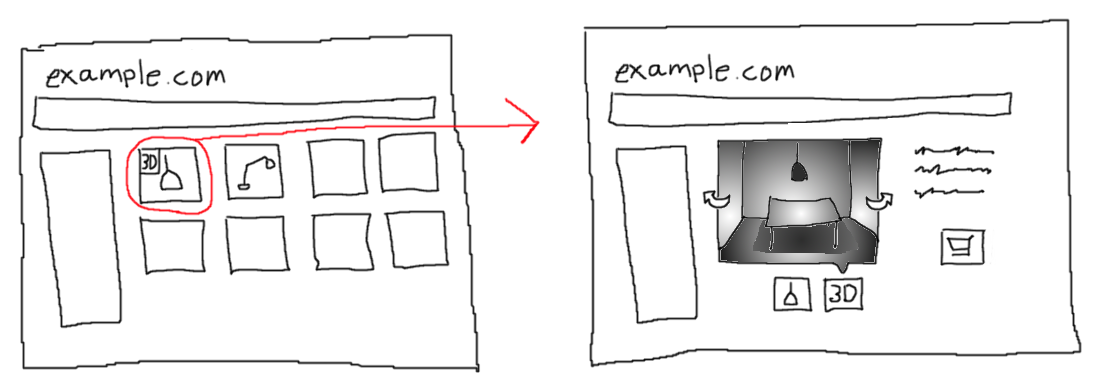
\includegraphics[width=\textwidth]{skitse_til_loesning}
   \caption{Skitse af ide til løsning.}
   \label{fig:skitse_af_ide}
\end{figure}

På figur \ref{fig:skitse_af_ide} er der illusteret en skitse af en e-butik, som sælger lamper. Figuren illustrerer hvordan systemet kan integreres på en hjemmeside. Skitse \ref{fig:skitse_af_ide}a viser et online katalog over e-butikkens udvalg af lamper. Som det fremgår af skitsen vil nogle lamper være markeret med et "3D-ikon" og dette indikerer, at kunden har mulighed for, at se lampen fra flere vinkler. Kunden tilgår billedet ved at klikke på ikonet. Når kunden trykker på ikonet bliver kunden omdirigeret til en anden menu. Som det fremgår af skitse \ref{fig:skitse_af_ide}b, så har kunden her mulighed for at se en billede af lampen. De to pile på skitsen indikerer, at kunden har mulighed for at rotere billedet, og se hvordan belysningen fra lampen er, set fra forskellige vinkler. Som en ekstra feature har kunden mulighed for at vælge en kontekst, som gør det muligt at se hvordan lampen ser ud i den kontekst som kunden ønsker at bruge lampen i. 
Derudover har kunden mulighed for, at justere lampens farvetemperatur i kelvin. Meningen med denne feature er, at kunden har mulighed for at visualisere hvordan forskellige pærer vil se ud i lampen. De forskellige billeder for lampen fra forskellige synsvinkler og farvetemperaturer, vil ligge til rådighed på en ekstern server og vil derfor ikke gøre e-butikkernes hjemmeside betydeligt langsommere. 

\begin{figure}[H]
  \center
  \begin{tikzpicture}
    \foreach \x in {0,5,10}
      \draw [black, thick] (\x, 0) -- (\x, -5.5);
    
    \node [above] at (0,0)  {Kunde};
    \node [above] at (5,0)  {E-butik};
    \node [above] at (10,0) {Server};

    \node [above] at (2.5, -0.5-0.1) {\small Besøger e-butik};
    \draw [black, thick, -{Stealth[width=3mm, length=3mm]}] (0,-0.5) -- (5,-0.5);
    \node [above] at (2.5, -1.0-0.1) {\small Lampekatalog};
    \draw [black, thick, -{Stealth[width=3mm, length=3mm]}] (5,-1.0) -- (0,-1.0);
    \node [above] at (2.5, -1.5-0.1) {\small Valg af lampe};
    \draw [black, thick, -{Stealth[width=3mm, length=3mm]}] (0,-1.5) -- (5,-1.5);
    \node [above] at (7.5, -2.0-0.1) {\small Anmod om billede};
    \draw [black, thick, -{Stealth[width=3mm, length=3mm]}] (5,-2.0) -- (10,-2.0);
    \node [above] at (7.5, -2.5-0.1) {\small Valg af lampe};
    \draw [black, thick, -{Stealth[width=3mm, length=3mm]}] (10,-2.5) -- (5,-2.5);
    \node [above] at (2.5, -3.0-0.1) {\small Billede};
    \draw [black, thick, -{Stealth[width=3mm, length=3mm]}] (5,-3.0) -- (0,-3.0);
    \node [above] at (2.5, -3.5-0.1) {\small Billede};
    \draw [black, thick, -{Stealth[width=3mm, length=3mm]}] (0,-3.5) -- (5,-3.5);
    \node [above] at (7.5, -4.0-0.1) {\small Skift vinkel og farvetemperatur};
    \draw [black, thick, -{Stealth[width=3mm, length=3mm]}] (5,-4.0) -- (10,-4.0);
    \node [above] at (7.5, -4.5-0.1) {\small Anmod om billede};
    \draw [black, thick, -{Stealth[width=3mm, length=3mm]}] (10,-4.5) -- (5,-4.5);
    \node [above] at (2.5, -5.0-0.1) {\small Billede};
    \draw [black, thick, -{Stealth[width=3mm, length=3mm]}] (5,-5.0) -- (0,-5.0);
  \end{tikzpicture}
   \caption{Sekvensdiagram af løsningsideen.}
   \label{fig:sekvensdiagram_af_ideen}
\end{figure}

Figur \ref{fig:sekvensdiagram_af_ideen} tager udgangspunkt i en hjemmeside, som har fået implementeret vores løsning, og viser et sekvensdiagram, som illustrerer processen når en kunde vil købe en lampe.  

I forbindelse med implementeringen af softwaren på en hjemmeside har der været forskellige ting, som skulle overvejes. Da problemet omhandler visualisering af lys fra lamper, er det primære mål at kunden kan se billeder af lampen og dens belysning fra forskellige synsvinkler og med forskellige farvetemperaturer. Derfor er muligheden for valg af konteksten anden prioriteret, når der skal udvikles en løsning. 

